% ----------------------------------------

\subsection{Contextual hypotesis}

% ----------------------------------------

\begin{frame}

\frametitle{Scenario}

In this case the e-commerce website doesn't register neither the \textbf{units sold} for each product nor the \textbf{class parameters}.

Since this isn't a change that affects the enviroment directly, there will not be a separate \textbf{masked environment} mask to hide the \textit{units sold} to the learner, therefore the extra information will be ignored by the learner.

We expect worse results overall since the learners are working with less data and therefore their prediction will have to factor in more \textbf{uncertainty}.

\end{frame}

% ----------------------------------------

\subsection{Algorithm}

% ----------------------------------------

\begin{frame}[fragile]

\frametitle{Algorithm}
\framesubtitle{Algorithm outline}

The learner that we modelled for this specific scenario bares a lot of \textit{similarities} w.r.t. the learner used for the previous step as they both function following the same workflow.

However, in this case, the \textbf{learn} function is only allowed to gather information from the generic reward obtained for the day.

\vspace*{1em}

\begin{lstlisting}[style=Python, basicstyle=\tiny, numbers=none]
def learn(self, _, reward: float, prediction: np.ndarray):
	for i, p in enumerate(prediction):
		prediction_index = np.where(self.budget_steps == p)[0][0]
		self.product_mabs[i].update(prediction_index, reward)
\end{lstlisting}

\end{frame}

% ----------------------------------------

\subsection{Results}

% ----------------------------------------

\begin{frame}[plain]

\frametitle{Single run reward and regret}
\framesubtitle{Thompson Sampling and UCB}

\begin{center}
	\hspace*{-1em}
	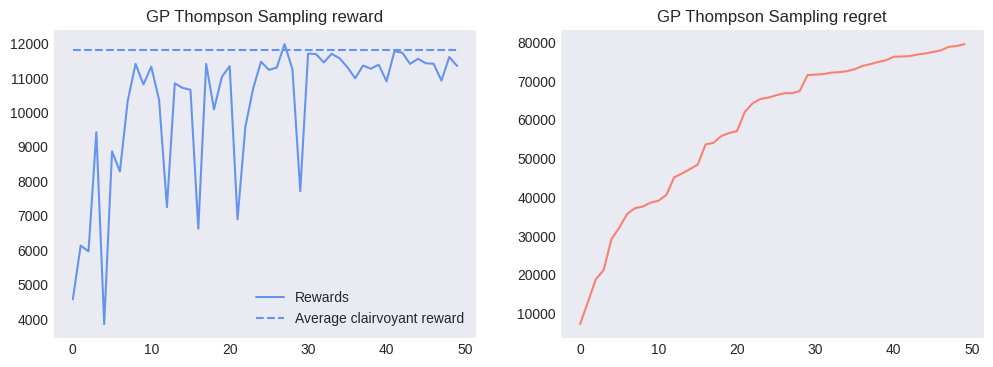
\includegraphics[scale=0.42]{img/Graphs/uncertain_alpha_unit/image1.png}
	\hspace*{-1em}
	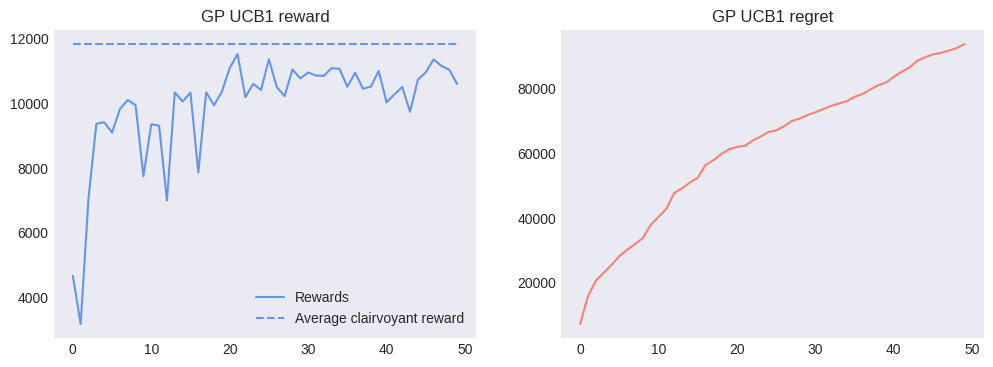
\includegraphics[scale=0.42]{img/Graphs/uncertain_alpha_unit/image2.png}
\end{center}

\end{frame}

% ----------------------------------------

\begin{frame}[plain]

\frametitle{Regret comparison}
\framesubtitle{Thompson Sampling and UCB}

\begin{center}
	\hspace*{-2.8em}
	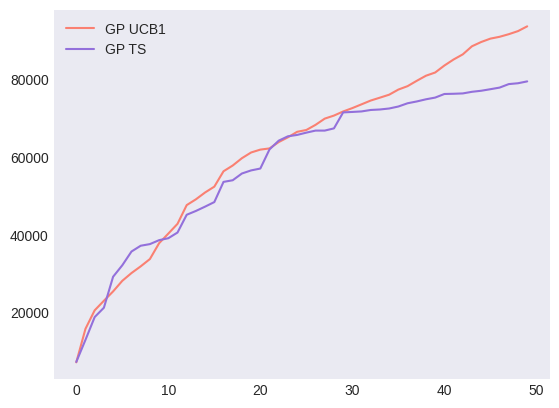
\includegraphics[scale=0.55]{img/Graphs/uncertain_alpha_unit/image3.png}
\end{center}

\scriptsize All tests are done using the \texttt{example\_environment} default values, \textit{population mean} of 1000, \textit{variance} of 10 and 20 \textit{budget steps}.

\end{frame}

% ----------------------------------------

\begin{frame}[plain]

\frametitle{Average reward and regret}
\framesubtitle{Thompson Sampling and UCB}

\begin{center}
	\hspace*{-1em}
	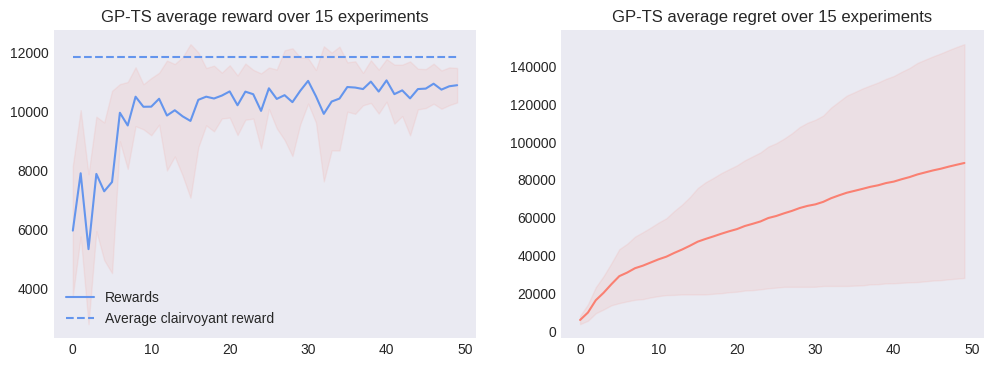
\includegraphics[scale=0.42]{img/Graphs/uncertain_alpha_unit/image4.png}
	\hspace*{-1em}
	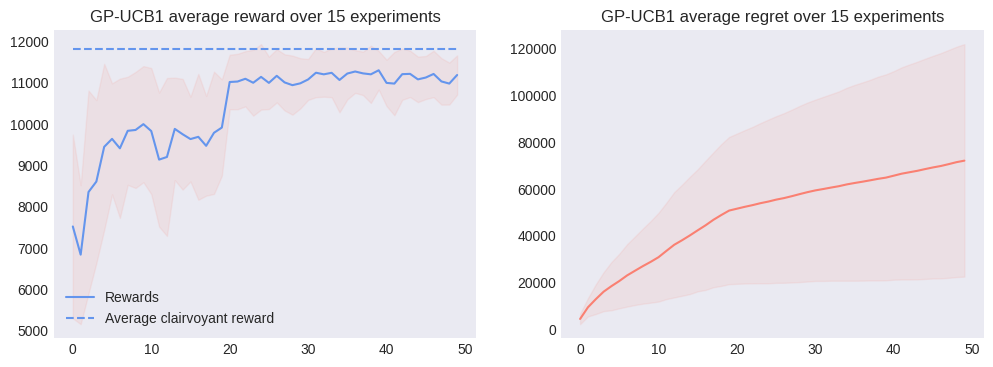
\includegraphics[scale=0.42]{img/Graphs/uncertain_alpha_unit/image5.png}
\end{center}

\end{frame}

% ----------------------------------------

\begin{frame}[plain]

\frametitle{Average regret comparison}
\framesubtitle{Thompson Sampling and UCB}

\begin{center}
	\hspace*{-2.8em}
	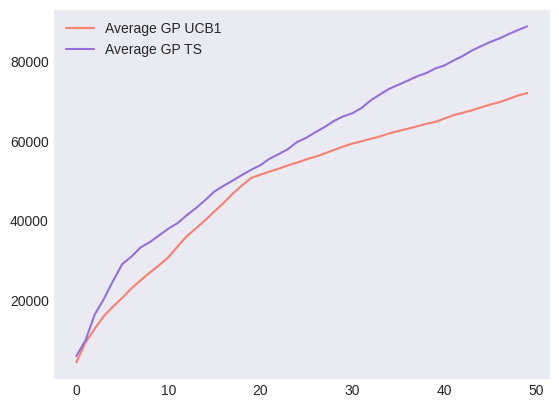
\includegraphics[scale=0.55]{img/Graphs/uncertain_alpha_unit/image6.png}
\end{center}

\end{frame}

% ----------------------------------------

\begin{frame}

\frametitle{Results}

In this scenario, results are worse w.r.t. the previous step since the learners work with less information.

\textbf{TS} seems to reach the optimal solution but is much more unstable than the previous case, however, if we use the \textbf{UCB} approach we are not guaranteed to find the optimal arm as sometimes it settles on a suboptimal solution.

On average we can observe that \textbf{UCB} performs slightly better than \textbf{TS} probably due to a more unrealiable environment resulting in learners that are more "unsure" nullifying the advantage dictated by the randomness of the latter.

\end{frame}

% ----------------------------------------

\begin{frame}

\frametitle{Results}

Average results over 15 runs at time horizon $T = 50$:

\begin{table}
	\begin{tabular}{|c|cc|c|}
	\hline \hline
		\cellcolor{blue!25} & Reward 	& Regret	& Deviation \\
	\cline{2-4}
		\cellcolor{blue!25} & $\mu$		& $\mu$		& $\sigma$	\\
	\hline \hline
		GPTS 				& 10772.60	& 97205.53	& 904.08	\\
	\hline
		GPUCB				& 11029.20	& 72557.20	& 510.36	\\
	\hline \hline
	\end{tabular}
\end{table}

\end{frame}

% ----------------------------------------
